\documentclass[fontset=ubuntu]{ctexart}
\usepackage[a4paper,margin=1in,headheight=13pt]{geometry}
\usepackage[hidelinks]{hyperref}
\usepackage{titlesec}
\usepackage{setspace}
\usepackage{fancyhdr}
\usepackage{enumitem}
\usepackage{textcomp}
\usepackage{graphicx}
\usepackage{booktabs}
\usepackage{array}
\usepackage{tabularx}
\usepackage{color}
\definecolor{darkblue}{rgb}{0.0,0.0,0.6}
\definecolor{cyan}{rgb}{0.0,0.6,0.6}
\usepackage{listings}
\lstset{
  language=C,
  basicstyle=\ttfamily,
  keywordstyle=\color{blue}\bfseries,
  commentstyle=\color{cyan},
  stringstyle=\color{red},
  showstringspaces=false,
  literate={--}{{\texttt{-{}-}}}2
}
\usepackage{biblatex}
\addbibresource{reference.bib}
\let\oldhref\href{}
\renewcommand{\href}[2]{\oldhref{#1}{\textit{#2}}}

\usepackage{titlesec}

\titleformat{\paragraph}
{\normalfont\normalsize\bfseries}{\theparagraph}{1em}{}
\titlespacing*{\paragraph}
{0pt}{3.25ex plus 1ex minus .2ex}{1.5ex plus .2ex}

% 调整段落间距
\setlength{\parskip}{6pt plus 2pt minus 1pt}

% 设置页码位置
\pagestyle{fancy}
\fancyhf{}
\rfoot{\thepage}
\renewcommand{\headrulewidth}{0.4pt} % 添加页眉下的横线
\lhead{\leftmark} % 在左侧页眉显示当前章节
\rhead{\rightmark} % 在右侧页眉显示当前小节

\title{操作系统实践指导 \\ \large Guide to Labworks by WQY}
\author{吴清晏 (61522314) \\ 东南大学吴健雄学院}

\date{}

\setcounter{tocdepth}{2}
\setcounter{secnumdepth}{3}
\begin{document}

\maketitle
\thispagestyle{empty}

\newpage
\renewcommand{\abstractname}{\LARGE\textbf{前言}}
\newgeometry{margin=1.2in}
\begin{abstract}\large
    \vspace{1cm}
    \noindent 感谢您使用《Guide to Labworks by WQY》!

    本文由吴健雄学院22级吴清晏编写,希望能帮助同学们顺利完成操作系统实验的准备工作,加深对操作系统的理解。

    首先,为使用Windows系统的同学提供了VMware虚拟机和WSL (Windows Subsystem for Linux)的安装教程,还包括实验文件与Xv6的下载以及运行环境配置。

    然后,以Reverse实验为例,说明了C语言实验的一般流程,包括需求分析,功能实现和测试等。

    最后,以Syscall实验为例,说明了Xv6实验的一般流程,包括Xv6系统的文件介绍等。

    值得注意的是,Mac系统自带Unix内核,不需要额外配置,但Mac系统的终端和Linux系统的终端有一些不同,需要注意一些命令的区别。据同学所说,Mac电脑上Xv6的运行可能存在一些问题,主要是因为安装qemu存在一定的困难。即使如此,考虑到Mac电脑的性能,我依旧不推荐使用虚拟机。

\end{abstract}
\thispagestyle{empty}
\restoregeometry{}

\newpage
\begin{center}
    \tableofcontents
\end{center}
\thispagestyle{empty}

\newpage
\pagenumbering{arabic}

\section{课前准备教程}

在开始前,请明确你是仅仅想完成《操作系统》的课程实验,还是想获得Linux的完整体验。考虑到大部分同学已经习惯了Windows系统的操作,我不推荐安装双系统,可通过Windows上的VMware体验带有图形桌面的Linux系统。VMware的性能有限,且在网络,硬件驱动等方面存在一定的配置难度,目前性能更高的解决方案是使用WSL (Windows Subsystem for Linux),但其不包含图形化桌面,大部分操作需要通过命令行进行,如果没有足够的信心,建议还是使用VMware。无论如何你都会需要的部分有:GNU编译环境安装,实验文件下载,Xv6配置。

\subsection{虚拟机配置}

在配置虚拟机前,需要先选择Linux发行版。推荐使用Ubuntu,它是最流行的Linux发行版之一,有着丰富的社区支持和软件资源。如果你对Linux有一定的了解,可以选择其他发行版,如Debian,Fedora等。对于WSL,只推荐其明确支持的发行版,其他发行版可能会出现一些问题,如CentOS的较早版本会缺少一些关键的库。

\subsubsection{VMware}

如果你需要运行带有图形界面的软件,那么VMware可以提供接近双系统的体验。网上有大量VMware的\href{https://zhuanlan.zhihu.com/p/617093823}{安装教程}。此外,还需要下载\textbf{.iso}格式的Linux安装镜像。推荐通过\href{https://mirrors.seu.edu.cn/}{东南大学镜像站}下载,建议选择\href{https://mirrors.seu.edu.cn/ubuntu-releases/22.04/ubuntu-22.04.4-desktop-amd64.iso}{Ubuntu22.04版本}。使用VMware的同学可跳过Git配置部分和其他配置部分。

\subsubsection{WSL + Ubuntu}

\noindent 目前仅Win10/11可使用WSL,其中Win11的配置较简单。以下是一般情况下的配置步骤\cite{microsoft2023}:

\begin{enumerate}
    \item “Win + r”打开“运行”,输入“control”打开“控制面板”,搜索或在“程序和功能”中选择“启动或关闭Windows功能”,勾选“适用于Linux的Windows子系统”和“虚拟机平台”。
    \item “运行”中输入“cmd”打开终端,在终端中输入“\texttt{wsl\ --update}”。Win11中会自动安装Ubuntu,Win10中需要输入“\texttt{wsl.exe\ --list\ --online}”列出所有可用发行版,推荐选择\texttt{Ubuntu}。安装成功后,Win10与Win11操作没有区别。
    \item 安装过程中,根据提示输入用户名和密码。用户名中不能出现英文大写,\textbf{密码默认隐藏}!
    \item 安装完成后,通过“\texttt{sudo\ passwd}”设置管理员密码,推荐采用与当前用户一样的密码,防止遗忘。为了防止误操作,平时尽量使用普通用户,需要管理员权限时使用“\texttt{sudo\ \textless{}command\textgreater{}}”。
    \item WSL默认安装到C盘,可通过在Windows终端中输入以下代码迁移到指定位置:
          \begin{lstlisting}
wsl --shutdown  # 关闭所有虚拟机
wsl --export Ubuntu <path>  # 导出虚拟机到指定位置
wsl --unregister Ubuntu  # 卸载原虚拟机
wsl --import Ubuntu <path> <new-path>  # 从刚刚位置导入虚拟机
    \end{lstlisting}

          以上步骤同样可用于保存虚拟机备份和在不同设备间迁移虚拟机。
\end{enumerate}

\noindent Tips:
\vspace{-0.5cm}
\begin{itemize}
    \item 如果近期重新安装过“Win11家庭版”系统,有可能报错\texttt{注册表缺失},最简单的方法是升级到\href{https://software.seu.edu.cn/soft/detail/18}{Win11专业版},安装完成后在“启动或关闭Windows功能”页面勾选“Hyper-V”,关闭并重新打开两个功能。
    \item 部分情况下Ubuntu默认登录为root用户。可通过以下操作创建有“sudo”权限的普通用户,并设为默认用户。该设置在下一次启动WSL时生效。
          \begin{enumerate}
              \item 通过“passwd”命令设置root密码。
              \item 通过“\texttt{adduser\ \textless{}username\textgreater{}}”添加用户。
              \item 通过“\texttt{adduser\ \textless{}username\textgreater{}\ sudo}”给新用户添加管理员权限。
              \item 在Windows终端输入“\texttt{ubuntu\ config\ --default-user\ \textless{}username\textgreater{}}”
          \end{enumerate}
\end{itemize}

\subsection{GNU编译环境安装}

\begin{enumerate}
    \item 输入“sudo apt-get update”更新软件源列表
    \item 输入“sudo apt-get install build-essential gdb”安装GNU编译环境和调试工具
\end{enumerate}

\noindent Tips:
\vspace{-0.5cm}
\begin{itemize}
    \item build-essential包括了gcc,g++和make,其中gcc和g++分别为c和c++的编译器,make可以编译带有makefile文件的开源软件代码,后续将安装的qemu就通过make编译并启动。
    \item GDB的全称是GNU Debugger,VS code等IDE提供的断点调试等功能就是基于GDB的。
\end{itemize}

\subsection{文本编辑器或IDE安装}

文本编辑器仅支持最基本的功能,如代码高亮和自动格式化等。IDE可以运行和调试代码,但过于复杂。VS code介于两者之间,其功能比文本编辑器强大,但学习成本比IDE低。更重要的是,WSL原生支持VS code,更符合Windows使用习惯。

\subsubsection{文本编辑器}

Ubuntu系统已默认安装了vim和nana,在终端中输入“vim”或“nano”即可打开。vim是一个上限很高的文本编辑器,但仅支持键盘控制,习惯鼠标操作的Windows用户可能很难适应。nano是一个更简单的文本编辑器,所有需要的快捷键会显示在页面底部,适合初学者使用。

这两款文本编辑器都是面向命令行的,面向图形界面的文本编辑器往往与图形界面共同安装,但WSL也支持Gnome文本编辑器等图形界面内置工具。

Gnome文本编辑器的安装方式是“sudo apt install gnome-text-editor -y”,安装成功后可通过“gnome-text-editor <file-name-or-path>”打开指定文件。该文本编辑器类似Windows上的记事本,支持鼠标操作,但功能较为简单。

\subsubsection{Visual Studio Code}

VS Code是一款由微软开发的轻量级代码编辑器,支持多种编程语言,拥有丰富的插件和主题。安装步骤如下:

\begin{enumerate}
    \item 先在Windows中\href{https://code.visualstudio.com/insiders/}{安装VS code},推荐选择“System Installer”版本。安装时建议勾选“添加到右键菜单”。安装完成后,打开VS code,点击左侧扩展按钮,搜索“Chinese”,安装中文语言插件。网络上有大量VS Code的配置教程,这里不做详细介绍。
    \item 在wsl中输入“code\ .”,注意中间有空格。这行命令在当前目录下打开VS Code,首次运行会自动完成VS Code的初始化。% chktex 26
    \item 在VS Code窗口的顶部菜单选择“文件”$\rightarrow$“打开文件夹”,输入“\~{}”,“\~{}”代表个人目录。
    \item 通过VS Code左侧工具栏的资源管理器创建文件“helloworld.c”,输入以下代码:
          \begin{lstlisting}
#include <stdio.h>
int main(int argc, char *argv[])
{
    printf("Hello World\n");
    return 0;
}
          \end{lstlisting}
          保存后,在左侧工具栏选择“运行和调试”,选择 (GDB/LLDB) C/C++,点击绿色的三角形运行代码。期间,需要根据提示安装C/C++扩展。运行时,会自动打开底部集成终端,终端已经打开了两个窗口:
          \begin{enumerate}
              \item C/C++: gcc生成活动文件

                    \textasteriskcentered{}正在执行任务: C/C++: gcc 生成活动文件

                    正在启动生成$\ldots$

                    /usr/bin/gcc -g /home/july/helloworld.c -o /home/july/helloworld

                    生成已成功完成。

                    \textasteriskcentered{}终端将被任务重用,按任意键关闭。
              \item cppdbg: helloworld
                    \begin{figure}[htbp]
                        \centering
                        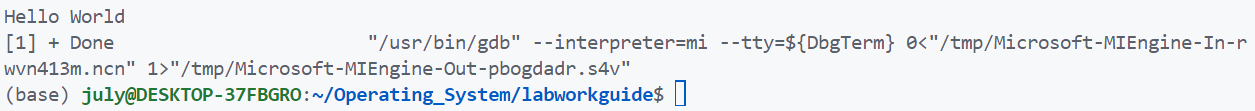
\includegraphics[width=\textwidth]{./README.assets/cppdbg.png}
                        \caption{cppdbg: helloworld}
                    \end{figure}
          \end{enumerate}
          如果输出与上图相同,说明GCC编译器和GDB调试器已经安装成功,VS Code的C/C++扩展也已经安装成功。
\end{enumerate}

\newpage{}

\subsection{Git配置}

Git是一个分布式版本控制系统,我们的Xv6下载就是通过Git进行的。Git的安装步骤如下:

\begin{enumerate}
    \item 在Windows上,\href{https://git-scm.com/downloads}{下载Git},安装时建议全部保持默认选项。
    \item 如果后续希望在GitHub上托管代码,还需要配置用户名和邮箱。在终端中输入以下命令:
          \begin{lstlisting}
git config --global user.name "Your Name"
git config --global user.email "youremail@domain.com"
        \end{lstlisting}
    \item 在wsl中输入“sudo apt-get install git”安装git。
\end{enumerate}

\subsection{其他配置}

这一部分是非必须的,但是有可能使后续操作更简单,看大家的需求。

\subsubsection{将VScode (WSL)添加到右键菜单}

在文件资源管理器中可右键选择通过Windows上的VScode打开当前文件夹。但是,对于WSL虚拟机中的文件,我们希望使用WSL上的VScode打开。此外,对于Windows 11,许多类似选项被放在了“更多选项”中,个人更习惯Windows7风格的右键菜单。可通过修改注册表自定义右键菜单,修改前建议备份注册表,具体步骤见\href{https://zhuanlan.zhihu.com/p/695724154}{教程}。

\subsubsection{在WSL中安装Chrome浏览器}

在实验文件中,有一些说明文档是html格式的,可以通过VS code查看,也可以选择在文件资源管理器中打开文件路径后,通过Windows上的浏览器打开。但是,如果一定想使用WSL中的浏览器,可根据官方提供的\href{https://learn.microsoft.com/zh-cn/windows/wsl/tutorials/gui-apps\#install-google-chrome-for-linux}{教程}操作。安装完成后,先不要着急打开浏览器,需要配置中文字体。如果现在直接打开,会出现大量警告信息,但配置完中文和输入法后大部分警告消失。剩余警告与Linux系统的省电模式有关,运行sudo apt-get install upower后警告完全消失\cite{wslissue2023}。

\subsubsection{配置中文与中文输入法}

如果你不习惯阅读英文报错信息,可以将Ubuntu的命令行语言设为英文\cite{monkeywie2021}。这不会影响输入命令的语法,只会影响一些报错和帮助信息的部分语句。你还可以安装中文输入法,并在刚刚安装的浏览器中使用。如果你没有安装任何WSL上的GUI应用,那么你不需要安装任何中文输入法。

\begin{enumerate}
    \item 输入“sudo apt install language-pack-zh-hans”安装中文语言包
    \item 输入“sudo dpkg-reconfigure locales”,在弹出窗口中选择en\_US.UTF-8和zh\_CN.UTF-8。空格键选择,回车键确认,ESC键退出。下一步的默认语言就是Ubuntu的命令行语言,推荐选择中文 (zh\_CN.UTF-8)
    \item 输入“sudo apt-get install fontconfig”安装字体配置工具
    \item 将Windows的字体文件链接到Ubuntu,具体方法是:
          \begin{enumerate}
              \item 输入“sudo vim /etc/fonts/local.conf”创建配置文件,按“i”进入编辑模式,输入以下内容:
                    \begin{lstlisting}[
                basicstyle=\ttfamily,
                columns=fullflexible,
                commentstyle=\color{gray}\upshape,
                stringstyle=\color{black},
                identifierstyle=\color{darkblue},
                keywordstyle=\color{cyan},
                morekeywords={xmlns,version,type}
              ]
<?xml version="1.0"?>
<!DOCTYPE fontconfig SYSTEM "fonts.dtd">
<fontconfig>
  <dir>/mnt/c/Windows/Fonts</dir>
  <dir>/usr/share/fonts</dir>
  <dir>/usr/local/share/fonts</dir>
  <dir prefix="xdg">fonts</dir>
</fontconfig>
              \end{lstlisting}

              \item 按“ESC”退出编辑模式,输入“:wq”保存并退出
          \end{enumerate}
    \item 输入“fc-cache -f -v”刷新字体缓存,并通过在Windows终端中输入wsl --shutdown和wsl来重启Ubuntu。注意,如果电脑中包含不止一个wsl环境,可以通过wsl --set-default <distro>设置默认环境,设置后可通过“wsl”命令打开默认环境。
    \item 输入“sudo apt install fcitx dbus-x11 im-config fcitx-sunpinyin adwaita-icon-theme-full”安装小企鹅输入法。
    \item 输入“sudo vim \~{}/.profile”,在文件末尾添加以下内容,退出方式与刚刚相同。
          \begin{lstlisting}[
            basicstyle=\ttfamily,
            columns=fullflexible,
            commentstyle=\color{gray}\upshape,
            stringstyle=\color{black},
            identifierstyle=\color{darkblue},
            keywordstyle=\color{cyan},
            morekeywords={export}
          ]
export GTK_IM_MODULE=fcitx
export QT_IM_MODULE=fcitx
export XMODIFIERS=@im=fcitx
export DefaultIMModule=fcitx
fcitx-autostart &>/dev/null
\end{lstlisting}
    \item 输入“source \~{}/.profile”应用配置。
    \item 输入“fcitx-config-gtk3”,现在应该能正常看到下图所示信息,说明配置成功。
          \begin{figure}[htbp]
              \centering
              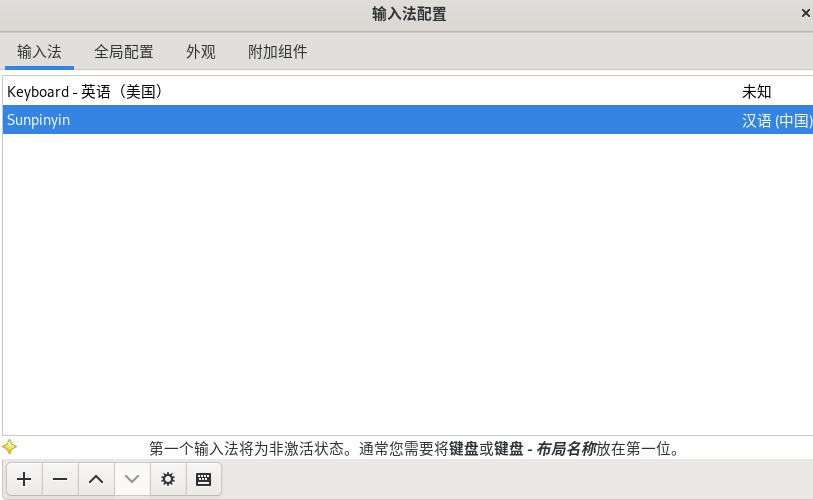
\includegraphics[width=0.6\textwidth]{./README.assets/fcitx.png}
              \caption{fcitx配置信息}
          \end{figure}
\end{enumerate}

\section{实验文件下载}

在下载实验文件前,请确保网络畅通,且可正常访问Github。如果无法稳定访问Github,可尝试“https://gitclone.com/”等镜像站点。

\subsection{Xv6实验}

\begin{enumerate}
    \item 从董恺老师提供的\href{https://seunic-my.sharepoint.cn/:u:/g/personal/101011912_seu_edu_cn/EUWd54wqsdJNu_h-sHQ1X2YBiZ24oi4rryRwXdoFGWpGsw?e=vDNOXc}{链接}下载实验文件夹,解压缩到WSL中的个人目录下 (如\~{}/projects)。
    \item 按照\href{https://www.overleaf.com/project/604ac6e691e6cf4d8ba0b24a}{实验指导书}的要求,完成普通实验,如Reverse。
    \item 对于Kernel-Hacking实验,在VS code集成终端中输入“cd \~{}/projects/Xv6-Syscall”。
    \item 输入“git clone https://github.com/mit-pdos/xv6-public.git”获取实验文件,网络顺畅的话,当前目录下会增加一个名为xv6-public的文件夹,将其改名为“src”。
    \item 输入“objdump -i”测试编译工具。若按照操作流程完成了GNU编译环境安装,应获得如下输出(语言可能存在差异,但请确保输出包含“elf32-i386”)。
          \begin{figure}[htbp]
              \centering
              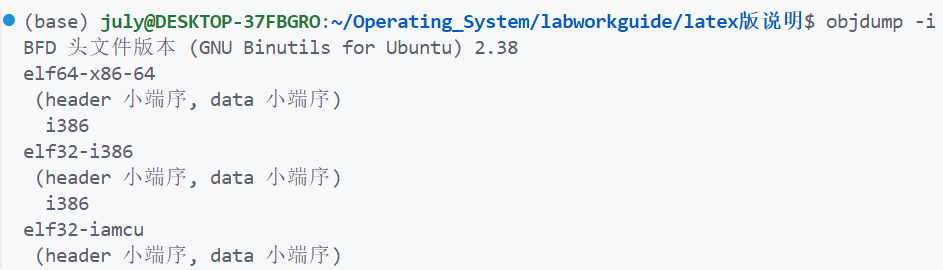
\includegraphics[width=\textwidth]{./README.assets/objdump.png}
              \caption{测试编译工具输出}
          \end{figure}
    \item 输入“sudo apt-get install qemu-system”安装qemu虚拟机
    \item 输入“cd src”进入文件夹,再输入“make”编译。编译完成后,输入“make qemu”运行Xv6系统。注意,以上过程均应在普通用户状态下执行,如果在root用户的个人目录下,会出现意料之外的权限问题。
\end{enumerate}

\newpage{}

\section{实验指南}

本部分旨在对\href{https://www.overleaf.com/read/bfhkrzwmhrrs}{《Guide to Xv6 Labworks》}中提到的两个实验进行说明,以帮助同学们了解实验的一般流程。希望大家先独立思考,如果遇到无法解决的问题,再尝试通过我的教程解决。

\subsection{Reverse实验}

在VS code中打开“\~{}”目录,在“./projects/Reverse”下新建“reverse.c”文件。

\subsubsection{需求分析}

\begin{enumerate}
    \item 支持3种输入形式:
          \begin{enumerate}
              \item \texttt{./reverse}
              \item \texttt{./reverse input.txt}
              \item \texttt{./reverse input.txt output.txt}
          \end{enumerate}
    \item 对于输入的数据 (命令行/文件),\textbf{不能}假设句子长度和句子个数。
    \item 处理以下4种错误:
          \begin{enumerate}
              \item 输入参数过多:“usage: reverse <input> <output>”
              \item 文件无法打开:“reverse: cannot open file <filename>”(<filename>为打不开的文件名)
              \item 输入相同文件:“reverse: input and output file must differ”(不能仅通过文件名判断)
              \item 内存分配失败:“malloc failed”
          \end{enumerate}
          用“fprintf(stderr, <error message>\textbackslash{}n);”输出错误并“exit(1);”返回状态码1。% chktex 36
\end{enumerate}

\noindent Tips:
\vspace{-0.5cm}
\begin{itemize}
    \item 其中,stderr是一种特殊的输出流,与之类似的输出流是stdout,stdout类似c++中cout。
    \item 返回的状态码正常为0,调用exit函数会立即终止并返回指定状态码。
\end{itemize}

\subsubsection{功能实现}

\begin{lstlisting}
    #include <stdio.h>
    #include <stdlib.h>
    #include <sys/stat.h>
\end{lstlisting}

\begin{enumerate}
    \item 处理错误“输入参数过多”
          \begin{lstlisting}
// reverse参数过多时打印usage: reverse <input> <output>并返回1
if (argc > 3) {
    fprintf(stderr, "usage: reverse <input> <output>\n");
    exit(1);
}	
    \end{lstlisting}
    \item 处理错误“文件无法打开”
          \begin{lstlisting}
// 输入流和输出流指针
FILE *input = stdin, *output = stdout;
// 尝试打开输入文件
if (argc >= 2) {
    input = fopen(argv[1], "r");
    if (input == NULL) {
        fprintf(stderr,"reverse: cannot open file '%s'\n",argv[1]);
        exit(1);
    }
}
// 尝试打开输出文件
if (argc == 3) {
    output = fopen(argv[2], "w");
    if (output == NULL) {
        fprintf(stderr,"reverse: cannot open file '%s'\n",argv[2]);
        exit(1);
    }
}
          \end{lstlisting}
    \item 通过头文件”<sys/stat.h>”提供的stat函数处理错误“输入相同文件”
          \begin{lstlisting}
struct stat stat1, stat2;
stat(argv[1], &stat1);
stat(argv[2], &stat2);
if (stat1.st_ino == stat2.st_ino) {
    fprintf(stderr,"reverse: input and output file must differ\n");
    exit(1);
}
    \end{lstlisting}
          \noindent Tips:
          \vspace{-0.3cm}
          \begin{itemize}
              \item stat函数可获取文件的状态信息,其中st\_ino是文件的inode号,用于唯一标识文件。这样可以处理不同文件名对应相同文件的情况,如软链接。
              \item 在C语言中,函数传值常常通过引用参数实现,这与Python等语言使用多个返回值的习惯不同。这种方式的优点是可以减少内存开销,缺点是可能会使代码更难理解。
          \end{itemize}
    \item 处理错误“内存分配失败”
          \begin{lstlisting}
// 记录行数和初始容量
int capacity = 10;
char **lines = malloc(capacity * sizeof(char *));
if (lines == NULL) {
    fprintf(stderr, "malloc failed\n");
    exit(1);
}
          \end{lstlisting}
    \item 实现缓冲区满自动扩容
          \begin{lstlisting}
int num_lines = 0, 
size_t len = 0;
while (1) {
    if (num_lines == capacity) {
        capacity *= 2;
        lines = realloc(lines, capacity * sizeof(char *));
        if (lines == NULL) {
            fprintf(stderr, "malloc failed\n");
            exit(1);
        }
    }
    if (getline(&lines[num_lines], &len, input) == -1)
        break;
    num_lines++;
}
          \end{lstlisting}
          \noindent Tips:
          \vspace{-0.3cm}
          \begin{itemize}
              \item “getline”函数在“len”设置为0时,会自动扩充输入缓冲区并更新“len”参数。
              \item 如果想测试零参数下的效果,可通过“Ctrl+D”终止输入流,此时“getline”函数会返回-1。
          \end{itemize}
    \item 将所有句子逆序放入输出流,释放内存并关闭文件
          \begin{lstlisting}
for (int i = num_lines - 1; i >= 0; i--) {
    fprintf(output, "%s", lines[i]);
    free(lines[i]);
}

free(lines);

if (input != stdin)
    fclose(input);
if (output != stdout)
    fclose(output);
    \end{lstlisting}
          \noindent Tips:
          \vspace{-0.3cm}
          \begin{itemize}
              \item 用malloc分配的内存一定要主动调用free函数进行内存释放,以防止内存泄漏。在程序终止时,操作系统会自动回收所有已分配资源,但主动回收有助于养成更好的代码习惯。
              \item 文件操作完成后一定要调用fclose函数关闭文件,因为每个打开的文件会消耗一个文件描述符,文件描述符达到上限将无法打开新文件。
              \item 当你发现电脑上有程序在运行过程中内存占用越来越大,说明发生了内存泄漏,可尝试终止程序并重新打开,利用操作系统完成资源回收。
          \end{itemize}
\end{enumerate}

\subsubsection{编译文件并测试功能}

\begin{enumerate}
    \item 选中文件,右键“在集成终端中打开”
    \item 输入“gcc -o reverse reverse.c -Wall”进行编译
    \item 输入“sudo chmod 777 test-reverse.sh”对当前测试脚本的权限进行修改
    \item 输入“sudo chmod 777 ../tester/*”将其他测试脚本的权限设为最高 % chktex 26

          \noindent Tips:
          \vspace{-0.3cm}
          \begin{itemize}
              \item “-Wall”参数用于在编译时显示所有的警告信息,包括未使用的变量、未初始化的变量、可能的数组越界等潜在问题,有助于提高代码质量。
              \item 可以用“chmod +x”替代“chmod 777”,前者只添加了执行权限。
          \end{itemize}
    \item 输入“./test-reverse.sh”进行测试。如果一切顺利的话,你会看到以下结果:
          \begin{figure}[htbp]
              \centering
              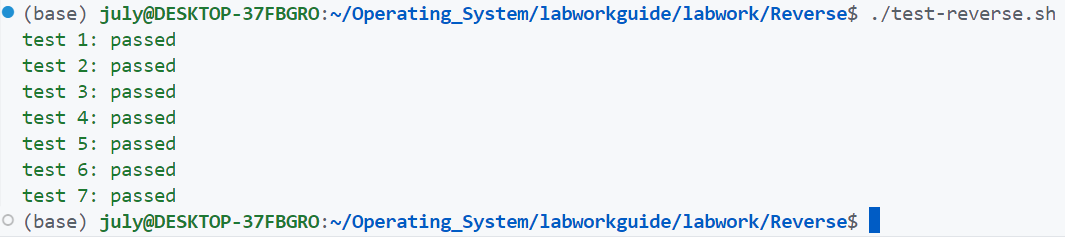
\includegraphics[width=\textwidth]{./README.assets/test-reverse.png}
              \caption{测试结果}
          \end{figure}
\end{enumerate}

\subsection{Syscall实验}

打开下载实验文件时创建的“src”文件夹,可看到“makefile”和大量“.c”,“.h”,“.S”文件,在“make”编译后额外出现了“.d”和“.o”文件。“.S”或“.s”是汇编文件的后缀名,其中“.S”后缀的文件支持预处理命令(如“\#”开头的大写命令)。% chktex 36

在进行系统调用的过程中,我们主要关心的文件有\cite{xv6official}:

\begin{center}
    \begin{tabularx}{0.8\textwidth}{>{\centering\arraybackslash}X >{\centering\arraybackslash}X}
        \toprule
        文件名    & 功能简介                     \\
        \midrule
        usys.S    & 提供用户态与内核态转换的接口 \\
        syscall.h & 定义系统调用号               \\
        syscall.c & 转发用户发起的系统调用到内核 \\
        sysfile.c & 实现系统调用                 \\
        sysproc.c & 另一种实现系统调用的选项     \\
        user.h    & 定义系统调用的参数传递方式   \\
        \bottomrule
    \end{tabularx}
\end{center}

接下来,我们将逐个分析这些文件,先观察系统原有的系统调用是如何实现的,再模仿原有的系统调用,实现“getReadCount”。当调用“getReadCount”时,返回read系统调用的总使用次数。

\newpage
\subsubsection{usys.S}

这个文件包含以下3个部分:

\begin{enumerate}
    \item 头文件
          \begin{lstlisting}
#include "syscall.h" // 包含每个系统调用对应的编号($SYS_ ## name)
#include "traps.h"   // 提供了($T_SYSCALL)的定义,此系统中为64。
    \end{lstlisting}
          \noindent 拓展信息:
          \vspace{-0.3cm}
          \begin{itemize}[listparindent=2em]
              \item \$T\_SYSCALL

                    在x86架构的计算机中,系统调用会触发一个陷阱(trap)。陷阱是一种特殊的中断,它会将CPU从用户态切换到内核态,并跳转到对应处理函数,函数地址由中断描述符表(IDT)提供,而\$T\_SYSCALL就是系统中断在IDT中的索引。
              \item IDT

                    IDT在“trap.c”中定义,是一个长度256的gatedesc数组。“gatedesc”在“mmu.h”中定义,这是一个结构体,包括“off\_15\_0”和“off\_31\_16”,他们合起来表示中断处理程序在其所在段的偏移地址,以及“cs”(处理函数所在段)和“args”(参数数量)等。
          \end{itemize}
    \item 宏定义接口模板

          “.\ globl name”使系统调用的名称成为全局变量,用户程序可以直接通过该名称进行系统调用。当该名称被使用时,自动把\$SYS\_ \#\# name放入“\%eax”,并发起“int”中断(“interupt”)。
          \begin{lstlisting}[language={[x86masm]Assembler}]
#define SYSCALL(name) \
  .globl name; \
  name: \
    movl $SYS_ ## name, %eax; \
    int $T_SYSCALL; \
    ret
    \end{lstlisting}
          \noindent 拓展信息:
          \vspace{-0.3cm}
          \begin{itemize}[listparindent=2em]
              \item \%eax

                    “eax”(Extended Accumulator Register)是16位“ax”的32位扩展。除“\%eax”寄存器外,汇编中还有“\%ebx”,“\%ecx”和“\%edx”,但不存在“\%eex”或“\%efx”等。实际上,“b”指“base”(基底),“c”指“counter”,“d”指“data”。

                    在x86架构的Linux中,“\%eax”负责传递系统调用的编号和执行完毕时的返回。
              \item int

                    大家可能会将其与c/c++中的int发生混淆。在汇编语言中,“int n”中“int”为“interrupt”指令的缩写,“n”为中断类型码。中断指令的执行往往包含以下步骤:
                    \begin{enumerate}
                        \item 指令指针(IP)和标志寄存器(FLAGS)入栈,其中FLAGS包含IF和TF
                        \item 查找IDT中对应的陷阱门,获取中断处理函数的段选择子和偏移地址
                        \item 将段选择子加载到代码段寄存器(CS),将偏移地址加载到指令指针(IP)
                        \item 执行完成时,通过“iret”指令弹出IP和FLAGS,恢复CPU状态。
                    \end{enumerate}
              \item “IF”(Interrupt Flag)

                    当“IF”为1时,允许响应可屏蔽中断。此处int指令会将IF设为0。

              \item “TF”(Trap Flag)

                    当“TF”为1时,CPU在执行每条指令后生成一个调试异常,通常用于单步调试。此处int指令会将TF设为0。
          \end{itemize}
    \item 通过宏定义模板声明系统调用

          已经完成的系统调用均采用“SYSCALL\(name\)”宏定义,在此基础上实现getreadcount:
          \begin{lstlisting}[language={[x86masm]Assembler}]
SYSCALL(getreadcount)
            \end{lstlisting}
          注意句尾无分号。
\end{enumerate}

下一步应该检查“syscall.h”和“traps.c”文件,并根据int指令的执行过程,寻找下一步须修改的文件。

\subsubsection{syscall.h}

该文件用于定义系统调用号。在最后增加getreadcount(void)对应的调用号,如“22”。 % chktex 36

\subsubsection{trap.c}

该文件定义了trap函数,其开始部分通过检查中断号类型判断是否为系统调用:

\begin{lstlisting}
    //PAGEBREAK: 41
    void
    trap(struct trapframe *tf)
    {
        if(tf->trapno == T_SYSCALL){
            if(myproc()->killed)
                exit();
            myproc()->tf = tf;
            syscall();
            if(myproc()->killed)
                exit();
            return;
        }
    }
\end{lstlisting}

当中断类型为系统调用时,将trapframe信息传递给myproc()并调用syscall()函数,该函数在“syscall.c”中定义。这里的myproc()函数通过pushcli和popcli调整中断禁用的深度,实现了某种锁,防止在获取当前进程信息时因为调度而错误地获取其他进程的信息。 % chktex 36

\subsubsection{syscall.c}

该文件提供了syscall()函数:% chktex 36
\begin{lstlisting}
    void syscall(void)
    {
        int num;
        struct proc *curproc = myproc();
      
        num = curproc->tf->eax;
        if (num > 0 && num < NELEM(syscalls) && syscalls[num]) {
          curproc->tf->eax = syscalls[num]();
        }
        else{
          cprintf("%d %s: unknown sys call %d\n",
                  curproc->pid, curproc->name, num);
          curproc->tf->eax = -1;
        }
    }
\end{lstlisting}

该函数用于将系统调用转发到内核。在该函数中,通过“tf-\textgreater{}eax”获取系统调用号,通过“syscalls[num]”获取对应的系统调用函数,执行该函数并将返回值存入“tf-\textgreater{}eax”中。

由此可见,我们需要在syscalls[]中增加getreadcount()函数的调用: % chktex 36
\begin{lstlisting}
    [SYS_getreadcount] sys_getreadcount
\end{lstlisting}

这时,出现了“未定义标识符 ``sys\_getreadcount''”报错,继续向上翻,我们还需要添加一行:

\begin{lstlisting}
    extern int sys_getreadcount(void);
\end{lstlisting}

这一行会告诉编译器,我们已经在其他文件中定义了该函数,编译器会自动去寻找。但编译器并没有找到“sys\_getreadcount”的函数定义,警告依然存在。

其他系统调用在“sysfile.c”或“sysproc.c”中定义,“sysfile.c”负责与文件相关的系统调用,如打开文件、读写文件、关闭文件等,“sysproc.c”负责与进程管理相关的系统调用,如创建进程、结束进程、等待进程等。

“getreadcount”被调用后会返回“read”的调用次数,个人认为它应该被归类为文件操作,但你也可以选择在“sysproc.c”中完成函数的定义,对于操作系统来说这两种方式没有区别。

\subsubsection{sysfile.c}

这个部分留给大家自己完成,你可以定义一个全局变量,每次调用“read”时自增,然后在“getreadcount”中返回该变量的值。

\subsubsection{user.h}

这个文件很多人可能会漏掉,它的作用是向用户提供该函数的接口。在其中增加一行:

\begin{lstlisting}
    int getreadcount(void);
\end{lstlisting}

这样能帮助c编译器检查系统调用传递的参数是否正确。

\subsubsection{测试功能}

在文件夹“Xv6-Syscal”中打开集成终端,并修改测试脚本权限:

\begin{lstlisting}[language=bash]
    sudo chmod 777 test-getreadcount.sh
    ./test-getreadcount.sh
\end{lstlisting}

正常情况下,因为在`getreadcount`实现部分没有对多线程进行针对性的处理,test2可能会无法通过,这是正常的。

\noindent Tips:

有使用VMware的同学在这一步出现了以下报错,可能是系统内置的包不同导致。
\begin{lstlisting}[language=bash]
    ./testgetreadcount.sh
    doing one-time pre-test (use -s to suppress)
    ../tester/xv6-edit-makefile.sh: line 6: gawk: command not found
    make: *** No rule to make target 'clean'.  Stop.
    make: Nothing to be done for 'xv6.img'.
    make: *** No rule to make target 'fs.img'.  Stop.
\end{lstlisting}

解决方法是手动安装缺少的包:
\begin{lstlisting}[language=bash]
    sudo apt-get install gawk
\end{lstlisting}


\newpage
\printbibliography{}

\end{document}
